\section{Additional GPU Validation Records}\label{app:gpu}
Table~\ref{tab:newcounts} compares historical and additional readouts.
The ARM dSprites mean is 54.0 rather than the historical HC count of 64.
The historical unnormalised CIFAR-10 ARD count was 14.2, but its
normalisation audit had already changed it to 26.0
(Table~\ref{tab:ard_normalized}). New exact-Jacobian counts are close
to that corrected result. Changes in training and prior updates prevent
attributing the full difference from 14.2 solely to the Jacobian calculation.
@@table52:pruning_counts@@

The new records comprise three seeds per dataset for ARM and for each
ARD variance-update setting. Gate bins in Table~\ref{tab:armgates} and
the individual constraint trajectories in Figure~\ref{fig:armconstraints}
show why a thresholded dimension count is insufficient to diagnose
successful pruning. In particular, dSprites does not approach a decisive
binary gate configuration or a satisfied constraint.
@@table52:arm_gates@@

\begin{figure}[!htbp]
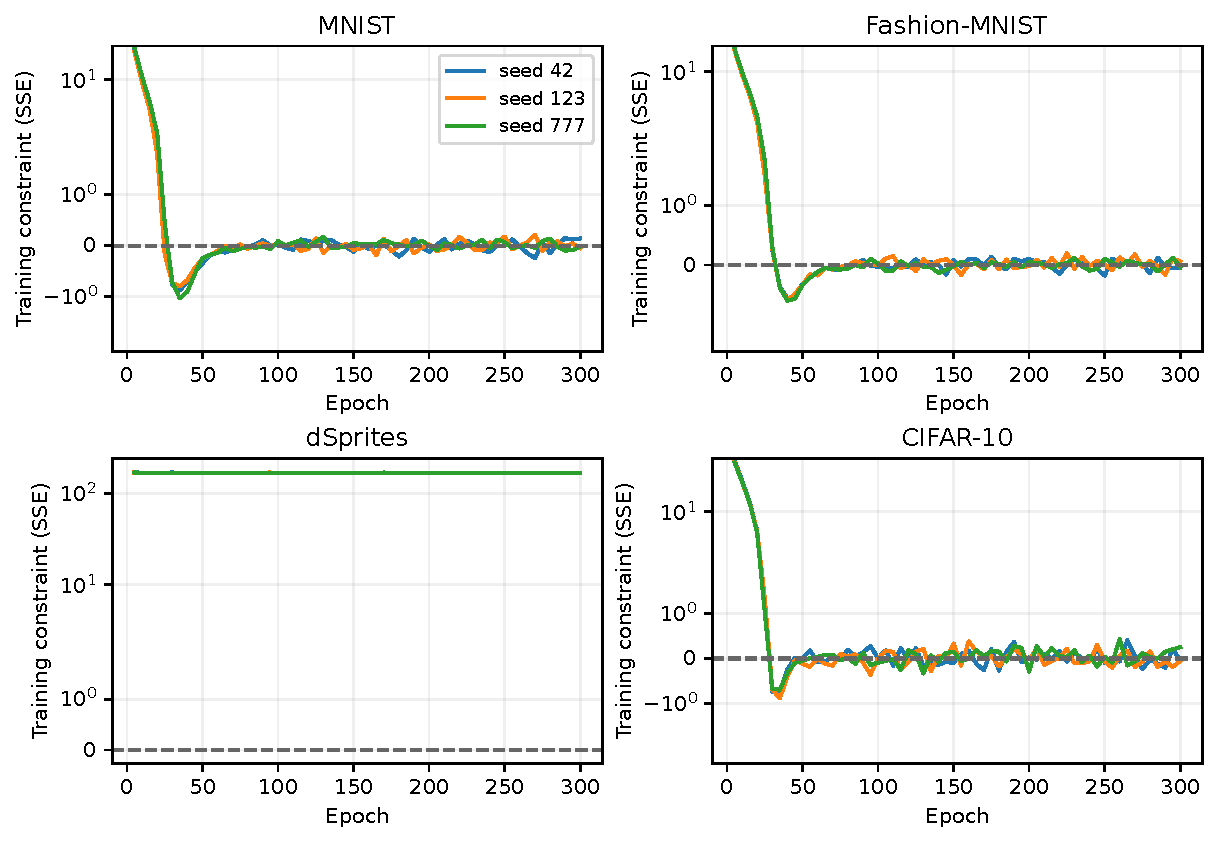
\includegraphics[width=\textwidth]{results/figures/MAKE52/arm_constraints.pdf}
\caption{Moving-average stochastic training constraint for each new ARM
seed, recorded every five epochs. Zero is the constraint boundary;
negative values satisfy it. A symmetric logarithmic vertical scale
accommodates large positive violations and negative values. These
trajectories are distinct from deterministic validation-target attainment.}
\label{fig:armconstraints}
\end{figure}

Figures~\ref{fig:armcurves} and~\ref{fig:ardcurves} report evaluation-mode
reconstruction curves for all four datasets. They describe the supplied
300-epoch runs; a visually flat curve does not certify an optimum.
The ARD figure uses zero-centre variance updates. All 24 ARD curve
records, including the sample-centred variant, are in the supplement.

\begin{figure}[!htbp]
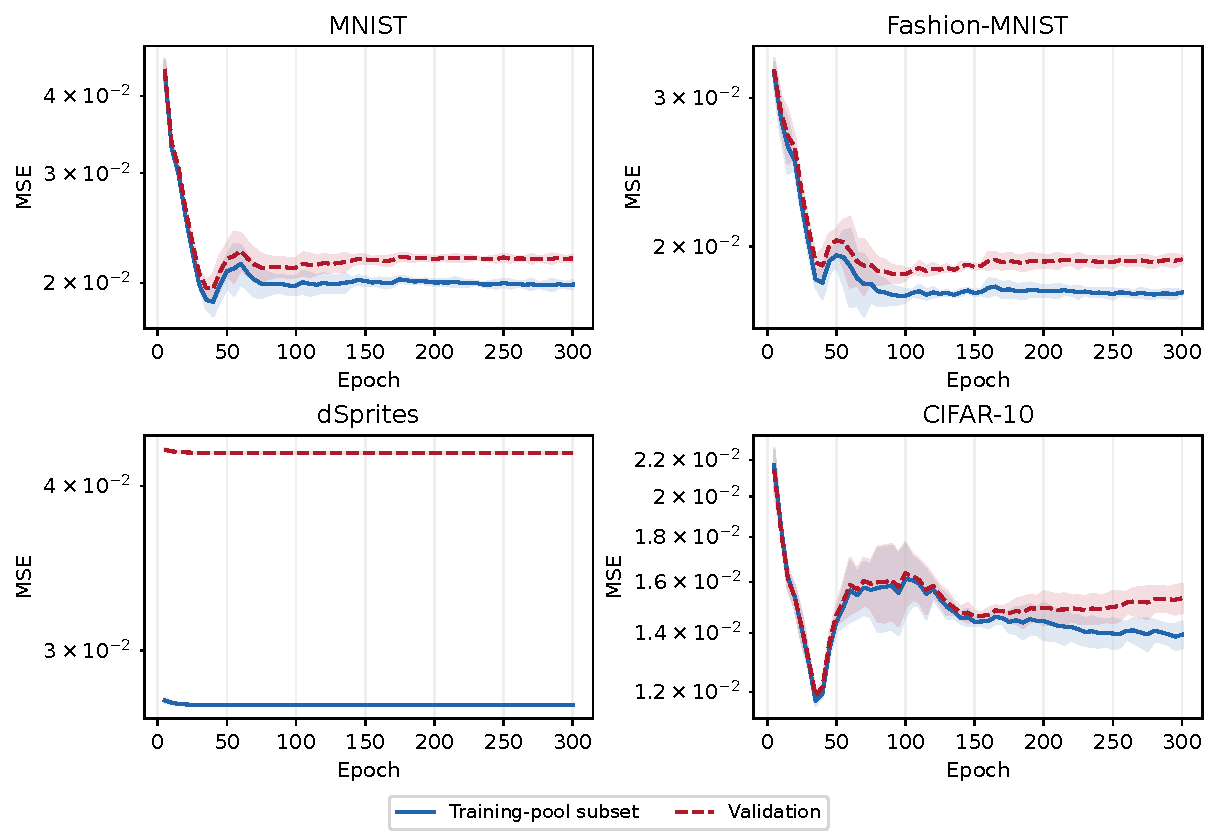
\includegraphics[width=\textwidth]{results/figures/MAKE52/arm_curves.pdf}
\caption{Native ARM posterior-mean MSE with the current binary gate mask,
evaluated every five epochs on a 2000-example training subset and the
validation split. Lines and shading are mean and sample SD over three
seeds. Vertical axes are logarithmic; a shaded lower bound is clipped
above zero for display. These curves do not reconstruct missing historical
ordinary-VAE training records.}
\label{fig:armcurves}
\end{figure}

\begin{figure}[!htbp]
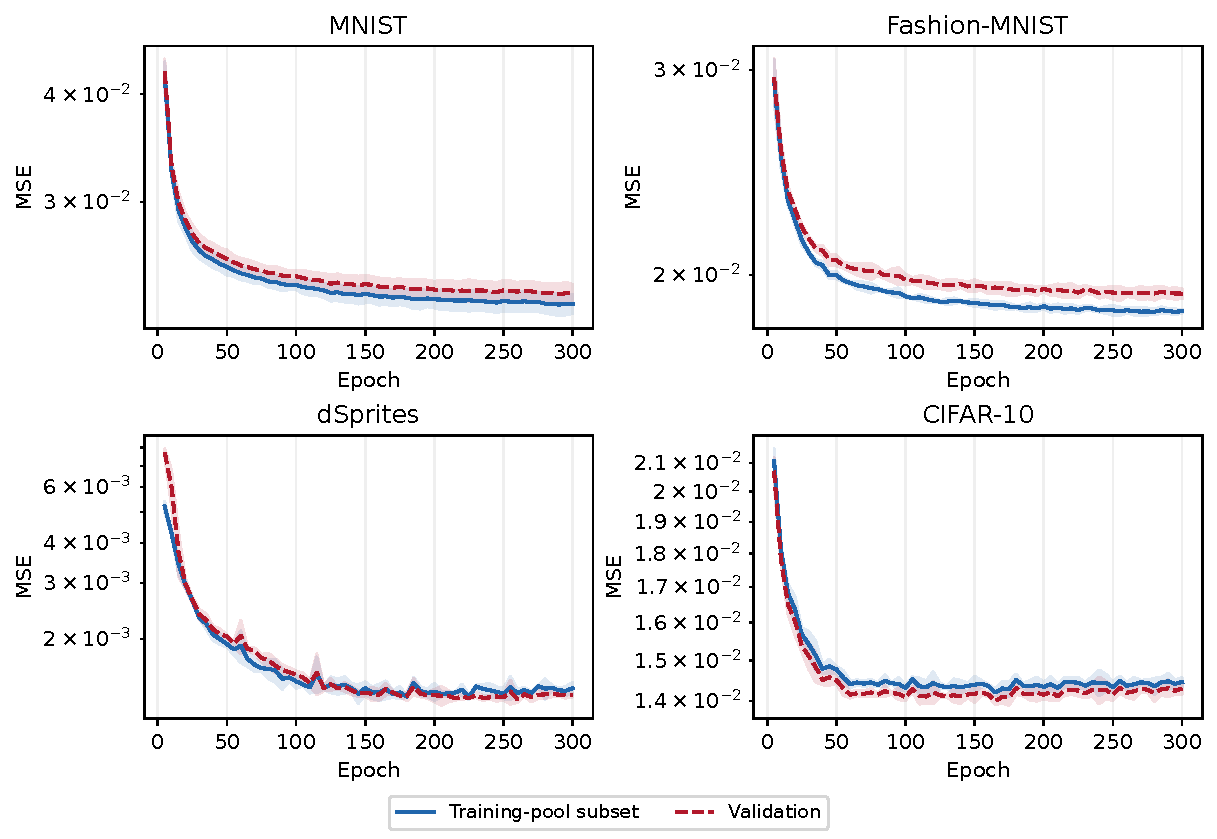
\includegraphics[width=\textwidth]{results/figures/MAKE52/ard_curves.pdf}
\caption{Full-width ARD posterior-mean MSE with zero-centre variance
updates, evaluated every five epochs. Mean and sample SD over three
seeds; logarithmic vertical axes. The 2000-example training-pool subset
includes 1800 examples reserved for prior updates and 200 used in
parameter-gradient training, so its curve is not a pure training-fit
estimate. No native pruning is applied in these evaluations.}
\label{fig:ardcurves}
\end{figure}

Table~\ref{tab:newtest} reports held-out test reconstruction at the
fixed final native models and transferred ordinary widths. Selection
uses the constraint or validation-based relevance readout, not these
test metrics. The full-model ARD column is deliberately distinguished
from quality at a selected native dimension.
@@table52:new_test@@

Table~\ref{tab:newcost} reports logged duration components. The source
records identify an NVIDIA GPU and the software environment. Training
intervals include periodic evaluation; the ARD initial and final prior
updates and final native evaluation are not included in the listed
training/Jacobian intervals. Jacobian timing pertains to 100 validation
examples and the particular architecture. Missing reference, anchor,
transfer and evaluation components preclude interpreting these numbers
as complete selector costs or combining them with historical CPU ID time.
@@table52:new_cost@@

\subsection{Native Masking and Decoder Adaptation}
Tables~\ref{tab:ardprunedseeds} and~\ref{tab:ardprunedtest} provide
the seed-level validation records and held-out test summaries for the
four native-pruning conditions. The selected counts match the preceding
sample-centred runs. Their unpruned validation/test MSEs are also
identical, so the repeated baseline is not extra independent evidence.
The dSprites test means follow the validation pattern: 0.00132 before
masking, 0.00294 after masking and 0.00178 after decoder adaptation.
@@table53:native_pruning_seeds@@

@@table53:native_pruning_test@@

Table~\ref{tab:ardprunedcost} reports the two recorded timing intervals.
Unlike the earlier curve runs, the initial training interval has no
periodic evaluation and includes the final prior update. The initial
prior update, Jacobian evaluation, mask construction and final model
evaluations are outside the recorded intervals. Adding training and
adaptation times would therefore not give end-to-end pruning cost.
The supplied script defines the 300-epoch training and 30-epoch
adaptation protocol, but its JSON lacks epoch counters and trajectories.
These settings are documented from the script and internal specification,
not independently recovered from a saved training trace.
@@table53:native_pruning_cost@@

The recorded \texttt{elbo} and \texttt{val\_elbo} fields remain in the
unmodified raw files for provenance but are not used as native ELBO
measurements (Section~\ref{sec:gpuvalidation}), including the new masking
records. Native post-masking MSE is now recorded, but checkpoints and
selected-axis identities were not saved. The mask, inference outputs
and a corrected native likelihood therefore cannot be independently
re-evaluated from the summaries alone. The analytic ARM-gradient check
validates a component; it cannot replace those model-level records.
